
\documentclass[]{article}

%\documentclass[]{svjour3}

\usepackage[german]{babel}
\usepackage[utf8]{inputenc}
\usepackage{mathtools}
\usepackage{moreverb}
\usepackage[colorlinks,bookmarksopen,bookmarksnumbered,citecolor=red,urlcolor=red]{hyperref}
\usepackage{relsize}
\usepackage{amsfonts}
\usepackage{mathrsfs}
\usepackage{subcaption}

\usepackage[table]{xcolor}
\usepackage{amsbsy}
\usepackage{mathrsfs}
\usepackage{amsmath}
\usepackage{amssymb}
\usepackage{longtable}

\usepackage{subcaption}
%\usepackage{algorithm}
\usepackage{algorithmicx}

\usepackage{autobreak} 
\usepackage{color}

\usepackage[]{algorithm2e}
\usepackage{graphicx}
\usepackage{amssymb}
\usepackage{color}
\usepackage{pgfplots}
\usepackage{subcaption}
\usepackage{paralist}
\captionsetup{compatibility=false}

\usepackage[numbers]{natbib}
\bibliographystyle{unsrt}
\usepackage{mathrsfs}
\usepackage{amsbsy}

\newtheorem{cond}{Conditions}%[section]


\newcommand{\matr}[1]{\mathbf{#1}}
\newcommand{\Qmat}{\matr{Q}}
\newcommand{\QDmat}{\matr{Q}_\Delta}
\newcommand{\tildeQDmat}{\matr{\tilde Q}_\Delta}
\newcommand{\todo}[1]{\textcolor{blue}{[TODO -- #1]}}
\newcommand{\vect}[1]{\boldsymbol{#1}}
\newcommand{\dt}{\Delta t}
\newcommand{\dx}{\Delta x}
\newtheorem{Condition}{Conditions}

\newcommand{\fcpre}{\hat{\matr{P}}}
\newcommand{\ccpre}{\tilde{\matr{P}}}
\newcommand{\fccp}{\matr{C}}
\newcommand{\cccp}{\tilde{\matr{C}}}

\newcommand{\fpre}{{\mathlarger{\mathscrbf P}}}
\newcommand{\sdcpre}{{\mathlarger{\mathscrbf P}}}
\newcommand{\cpre}{\tilde{ \mathlarger{\mathscrbf P}}}
\newcommand{\fcp}{{\mathlarger{\mathscrbf C}}}

\newcommand{\trans}{\mathlarger{\mathscrbf T}}
\newcommand{\rest}{{\mathlarger{\mathscrbf R}}}

\newcommand{\Ptimat}{\matr{\tilde{P}}}
\newcommand{\Phatmat}{\matr{\hat{P}}}
\newcommand{\iter}{\mathlarger{\pmb{\mathscr{I}}}}

\newcommand{\F}{\vect F}
\newcommand{\dF}{\nabla \vect F}
\newcommand{\AJ}{({\matr{A}/\dF})^*}
%\newcommand{\QDmat}{Q}


\setcounter{tocdepth}{3}
%\setcounter{secnumdepth}{3}
\newcounter{foo}

\begin{document}

\title{SDC and Reinforcement Learning}
\maketitle

\section{Aufgabenstellung}

Ziel: Löse das Kollokationsproblems
\begin{align}
C_f u = u_0 ,
\end{align}
mit Kollokationsoperator
\begin{align}
C_f (u) := (I_M \otimes I_N - \dt (Q \otimes I_N )f ) (u),
\end{align}
so effizient wie möglich.

Ansatz: Benutze den iterativen Löser SDC (eine vorkonditionierte Fixpunkti-
teration)
\begin{align}\label{sdc}
P_f(u^{k+1}) = P_f(u^k) + (u_0 - C_f (u^k )) \qquad \text{für } j = 0, 1, 2, . . . ,
\end{align}
mit
\begin{align}
P_f (u) := (I_M \otimes I_N - \dt (Q_\Delta \otimes I_N )f ) (u).
\end{align}
Frage: Wie ist die diagonale Matrix $Q_\Delta$ zu wählen um einen besonders guten
Vorkonditioniere $P_f$ zu erzeugen.

Wähle die Einträge $(q_\Delta)_{ii}$ von $Q_\Delta$ so, dass die Anzahl der Iterationen
von \eqref{sdc} bezüglich einer vorgegebenen Fehler-Schranke minimiert werden.


Im einfachsten Fall ist $u$ skalar und $f (u) = \lambda u$ wir nennen dies unsere Testgleichung und beschränken uns zunächst auf $\lambda \in [-100,0]$.





\section{Was bisher funtioniert: Konstante Matrix $Q_\Delta$}

\begin{itemize}
\item RL (unsere Implementierung): Eine Episode entspricht mehreren SDC-Iterationen \eqref{sdc}:
Für jede Iteration wird der Reward um eins verringert. Die Episode wird beended falls der Fehler eine vorgegebene Schranke ($10^{-10}$) unterschritten hat oder dies nach 50 Iterationen nicht der Fall ist. 	
\item MIN (Referenzlöser): Wir sind uns selbst nicht sicher wo diese Zahlen für $Q_\Delta$ herkommen
\item LU (Referenzlöser): Ist eine verbreitete Wahl von $Q_\Delta$ als untere Dreiecksmatrix
\end{itemize}

Wir benutzen unseren RL Agent (nach verschieden intensivem Training) um Testgeichungen mit verschiedenen $\lambda \in [-100,0]$ zu Lösen und vergleichen das Ergebnis mit den zwei anderen Lösern:\\

\begin{tabular}{| l | c | c | c | c | c |}
	\hline	
	Alg. und & durchschn Anz.& gef. Lösung für & gef. Lösung für & gef. Lösung für\\
	Länge Trainig & Iterationen	& $(q_\Delta)_{11}$ & $(q_\Delta)_{22}$ & $(q_\Delta)_{33}$\\
	              &             & $[min,max]$ & $[min,max]$ & $[min,max]$ \\
	              &             & $Mittel\pm Abw.$ & $Mittel\pm Abw.$ & $Mittel\pm Abw.$ \\
	\hline			
	RL 100k & 29.46 & $[0.329, 0.481]$ & $[0.179, 0.276]$ & $[0.0, 0.425]$ \\
	        &       & $0.423 \pm 0.009$ & $0.184 \pm 0.013$ & $0.401 \pm 0.078$\\
	\hline
	RL 1000k & 15.22 & $[0.255, 0.324]$ & $[0.128, 0.14]$ & $[0.302, 0.375]$ \\
	         &       & $0.318 \pm 0.008$  & $0.136 \pm 0.004$ & $0.34 \pm 0.009$  \\	
	\hline			
	MIN & 14.22 &  $0.320$ & $0.14$ & $0.372$ \\
	\hline  	
	LU &  11.53 & & &  \\
	\hline  
\end{tabular}\\

Die von RL gefundenen Werte für $Q_\Delta$ konvergieren gegen die MIN-Lösung (glaube ich).


\begin{figure}[h]
	\begin{minipage}[b]{.6\linewidth} % [b] => Ausrichtung an \caption
		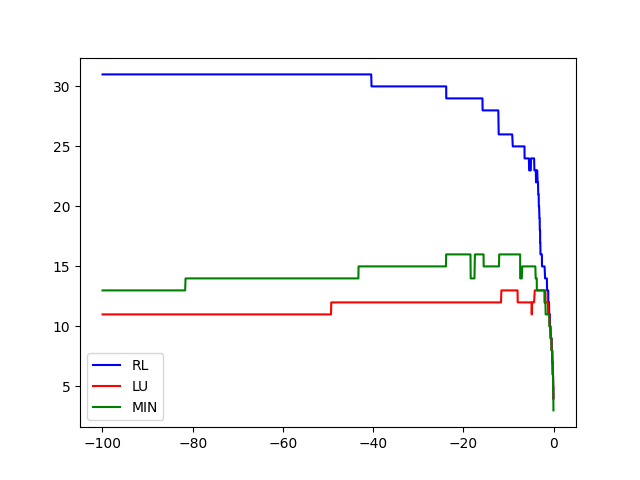
\includegraphics[width=\linewidth]{M_3_res_10_Lneg_100K_model_PPO2_v0.png}
		\caption{RL 100K}
	\end{minipage}
	%\hspace{.1\linewidth}% Abstand zwischen Bilder
	\begin{minipage}[b]{.6\linewidth} % [b] => Ausrichtung an \caption
		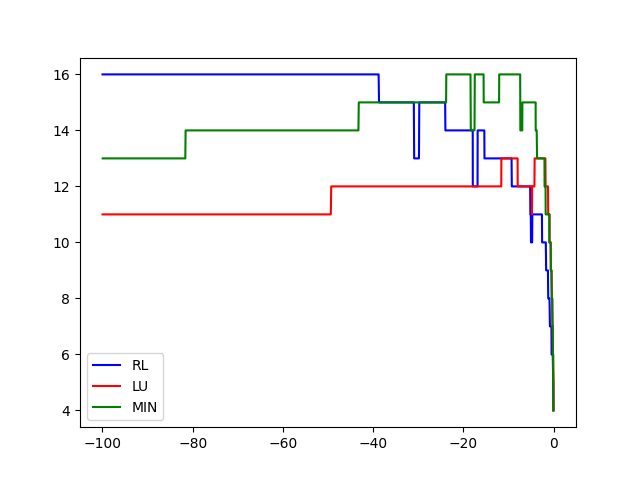
\includegraphics[width=\linewidth]{M_3_res_10_Lneg_1000K_model_PPO2_v0.png}
		\caption{RL 1000K}
	\end{minipage}
\end{figure}

\section{Bestimme $Q_\Delta$ in jeder Iteration}
Beschränke dazu das Training und die Auswertung auf $\lambda \in [-10,0]$.
(Für $\lambda=-20$ funktioniert das wirklich GAR NICHT aber vielleicht lerne ich auch nicht lange genug!)\\

Expertenrat: Benutze jetzt LSTM (Netzwerk war vorher vollständig verbunden) und finde eine passende Reward-Funktion:
\begin{itemize}
	 \item bisherige Belohnung: -1 für jede Iteration
	 \item jetzt abhängig vom Residuum $r^k$ und der gewünschten Genauigkeit $r_{tol}=10^{-10}$ und der Anfangsgenauigkeit $r^0$ 
	 \begin{align}
	 0.5*\frac{ log(r^k) - log(r^{k+1})}{log(r^0)-log(r_{tol})}-0.01
	 \end{align}
\end{itemize}
\begin{figure}[h]
	\begin{minipage}[b]{.6\linewidth} % [b] => Ausrichtung an \caption
		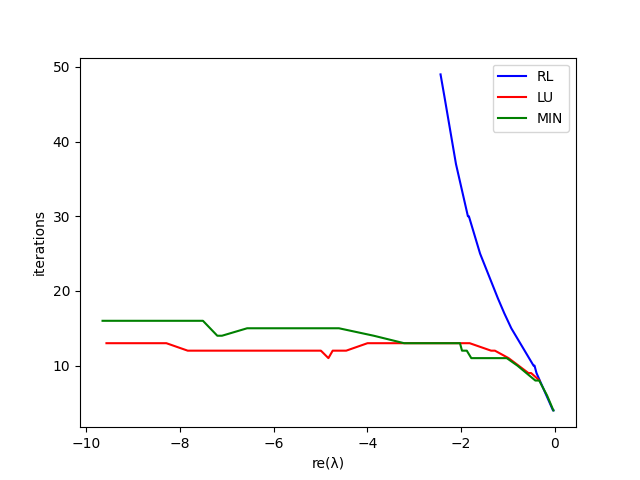
\includegraphics[width=\linewidth]{old.png}
		\caption{Reward wie bisher, 100K}
	\end{minipage}
	%\hspace{.1\linewidth}% Abstand zwischen Bilder
	\begin{minipage}[b]{.6\linewidth} % [b] => Ausrichtung an \caption
		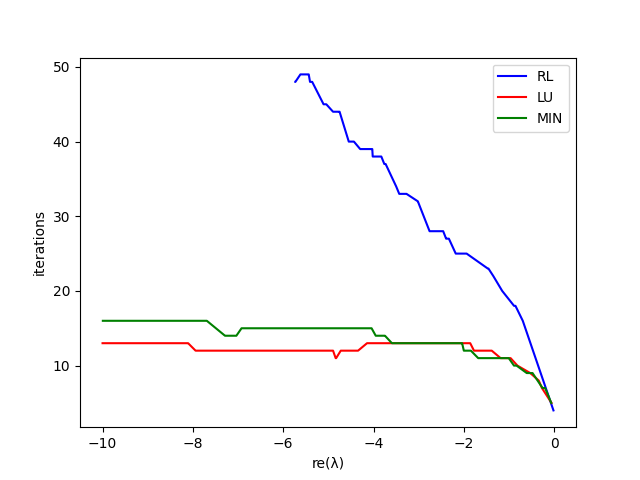
\includegraphics[width=\linewidth]{old1000.png}
		\caption{Reward wie bisher, 1000K}
	\end{minipage}\\
	\begin{minipage}[b]{.6\linewidth} % [b] => Ausrichtung an \caption
	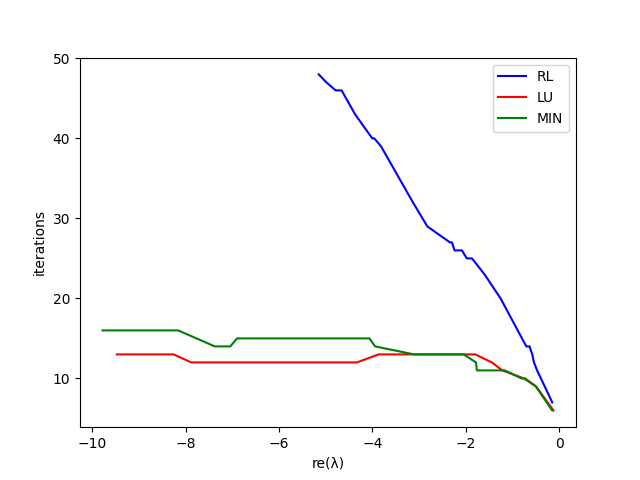
\includegraphics[width=\linewidth]{new.png}
	\caption{neuer Reward, 100K}
\end{minipage}
%\hspace{.1\linewidth}% Abstand zwischen Bilder
\begin{minipage}[b]{.6\linewidth} % [b] => Ausrichtung an \caption
	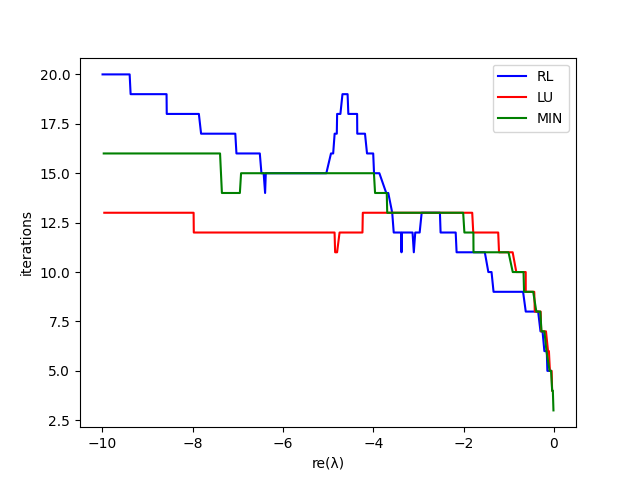
\includegraphics[width=\linewidth]{supertollnew.png}
	\caption{neuer Reward, 1000K}
\end{minipage}
\end{figure}

Die Matrix $Q_\Delta$, die von RL in Abbildung 6 verwendet wird lautet \\
$[0.612\pm 0.11,  0.307\pm 0.075, 0.0252 \pm 0.0282]$. 
%python rl_playground.py --policy_class='MlpLstmPolicy' --envname='sdc-v1' --tests=500 --steps=1000000 --num_envs=1
%Qd_11
%Mittel  0.612246033102274
%Abweichung  0.11016499313355534
%Maximum 0.7988364994525909
%Minimum  0.36844414472579956
%Qd_22
%Mittel  0.3065583620071411
%Abweichung  0.07514956695147787
%Maximum 0.4186137989163399
%Minimum  0.14376986026763916
%Qd_33
%Mittel  0.02520696723461151
%Abweichung  0.028179209519591474
%Maximum 0.0711229145526886
%Minimum  0.0
%RL  -- Mean number of iterations and success rate: 14.38, 100.0 %
%LU  -- Mean number of iterations and success rate: 11.98, 100.0 %
%MIN  -- Mean number of iterations and success rate: 13.73, 100.0 %

%Qd_11
%Mittel  0.5831997407209129
%Abweichung  0.08916154583006174
%Maximum 0.7084390670061111
%Minimum  0.41401416808366776
%Qd_22
%Mittel  0.286887083530426
%Abweichung  0.04999660884443219
%Maximum 0.34963780641555786
%Minimum  0.17471247911453247
%Qd_33
%Mittel  0.03128814446926117
%Abweichung  0.031873371246591314
%Maximum 0.08370944857597351
%Minimum  0.0
%RL  -- Mean number of iterations and success rate: 14.47, 100.0 %
%LU  -- Mean number of iterations and success rate: 12.04, 100.0 %
%MIN  -- Mean number of iterations and success rate: 13.77, 100.0 %
%passt zu neuer Reward 1000K
%python rl_playground.py --policy_class='MlpLstmPolicy' --envname='sdc-v1' --tests=500 --steps=1000000 --num_envs=1

%%%%%%%%%%%%%%%%%%%%%%%%%%%%%%%%%%%%%%%%%%%

%versuche jetzt alte Reward noch mal
%Qd_11
%Mittel  0.6129034758843481
%Abweichung  0.44774932343688606
%Maximum 1.0
%Minimum  0.0
%Qd_22
%Mittel  0.8922724523097276
%Abweichung  0.1967132112363039
%Maximum 1.0
%Minimum  0.3745957016944885
%Qd_33
%Mittel  0.11823945376649499
%Abweichung  0.168705005091214
%Maximum 0.5985580459237099
%Minimum  0.0
%RL  -- Mean number of iterations and success rate: 31.04, 52.6 %
%LU  -- Mean number of iterations and success rate: 12.06, 100.0 %
%MIN  -- Mean number of iterations and success rate: 13.74, 100.0 %
%Testing took 31.76271292200545 seconds.
\end{document}


